

\documentclass[conference]{IEEEtran}

\usepackage{adjustbox}
\usepackage{graphicx}
\usepackage{alphalph}

\let\OLDitemize\itemize
\renewcommand\itemize{\OLDitemize\addtolength{\itemsep}{1em}}
\let\OLDenumerate\enumerate
\renewcommand\enumerate{\OLDenumerate\addtolength{\itemsep}{1em}}
\renewcommand\thesubsectiondis{\AlphAlph{\value{subsection}}.}% for the headings in the text
\renewcommand\thesubsection{\mbox{\thesection-\AlphAlph{\value{subsection}}}}% for the ToC, for example     


% correct bad hyphenation here
\hyphenation{op-tical net-works semi-conduc-tor}


\begin{document}

\title{Assignment Helper\\ Empowering Your Programming Skill \\ Power OVERWHELMING co.}

% author names and affiliations
% use a multiple column layout for up to three different
% affiliations
% \author{\IEEEauthorblockN{Jae-gook Kim}
% \IEEEauthorblockA{Department of Information System\\
% Hanyang University, Seoul,  Korea\\
% Email: claretta@hanyang.ac.kr}
% \and
% \IEEEauthorblockN{Kyung-min Kim}
% \IEEEauthorblockA{Department of Information System\\
% Hanyang University, Seoul,  Korea\\
% Email: kimkmhk@hanyang.ac.kr}
% \IEEEauthorblockN{Ji-hoon Lee}
% \IEEEauthorblockA{Department of Finance,\\ Business School,\\
% Hanyang University, Seoul,  Korea\\
% Email: 1equal2@hanyang.ac.kr}
% \and
% \IEEEauthorblockN{Kyo-ho Lee}
% \IEEEauthorblockA{Department of Information System\\
% Hanyang University, Seoul,  Korea\\
% Email: 1equal2@hanyang.ac.kr}}


% conference papers do not typically use \thanks and this command
% is locked out in conference mode. If really needed, such as for
% the acknowledgment of grants, issue a \IEEEoverridecommandlockouts
% after \documentclass

% for over three affiliations, or if they all won't fit within the width
% of the page, use this alternative format:
% 
\author{\IEEEauthorblockN{Ji-hoon Lee\IEEEauthorrefmark{1},
Jae-gook Kim\IEEEauthorrefmark{2},
Kyung-min Kim\IEEEauthorrefmark{3}, and
Kyo-ho Lee\IEEEauthorrefmark{4} }
\IEEEauthorblockA{\IEEEauthorrefmark{2}\IEEEauthorrefmark{3}\IEEEauthorrefmark{4}Department of Information System}
\IEEEauthorblockA{\IEEEauthorrefmark{1}Department of Finance, Business School}
\IEEEauthorblockA{Hanyang University, Seoul, Korea}
\IEEEauthorblockA{Email: \IEEEauthorrefmark{1}starypoc@hanyang.ac.kr,  \IEEEauthorrefmark{2}claretta@hanyang.ac.kr, \IEEEauthorrefmark{3}kimkmhk@hanyang.ac.kr, \IEEEauthorrefmark{4}1equal2@hanyang.ac.kr}}



\maketitle

\begin{abstract}
Assignment Helper is a program to help people who have difficulties with their programming language assignments. Assignment Helper will able to help the assignment by crawling the data from webs such as programmer forums and then find similar questions and related codes. It will also have a verification function and will check the codes by using CRC or other compilers. It shall check it by testing the input, output and the expectation all together.

\centering


\begin{table}[h]
\renewcommand{\arraystretch}{1.3}
\caption{Role Assignment}
\label{table_role}
\centering
\begin{adjustbox}{width=0.5\textwidth}
\small
\begin{tabular}{c||c||c}
\hline
\bfseries Role & \bfseries Name & \bfseries Task Description \\
\hline\hline
Developer Manager  & Kim Jae-gook & \parbox[t]{5cm}{Managing whole process of developing\\ the program. }\\
\hline
Users & Lee Ji-hoon & \parbox[t]{5cm}{Seeking for the usefulness compare\\ to other similar programs.}\\
\hline
Cutomers & Kim Kyung-min & \parbox[t]{5cm}{Finding out whether the project is \\ valuable.}\\
\hline
Developer & Lee Kyu-ho & \parbox[t]{5cm}{Implementing the program.}\\
\hline

\end{tabular}
\end{adjustbox}

\end{table}
\end{abstract}

\IEEEpeerreviewmaketitle


\section{Introduction}

\subsection{Motivation}
We have started this project with the motivation to help students (especially freshman) who are struggling with their assignments. Other assignments like history or natural science can easily find their assignment sources quickly from just googling it simply. However, it is impossible to do that simple procedure in programming language assignment. Without perfect knowledge about the computer languages, it comes out difficult to solve their programming language assignment. 

We discussed about a solution to solve this. We concluded that it is not easy to study programming languages especially to the students who studied only at school and have never lived closed to computer languages; The students who only studied subjects for KSAT, the entrance exam for university!

\subsection{Problem Statement}
It is problematic for those who first met the programming language and getting no additional help. It can be not only unfair but also can cause inefficiency in terms of the social resource allocation. Maybe, some novice students might have natural talents at computer programming. But others needs opportunities to catch up. So, we are going to build a program to ease the life of these novice students.


\subsection{Research on Any Related Software}
Our program aims for helping students who is unfamiliar with programming paradigms. There are some services which provide help to those students in primitive levels than our service.

\subsubsection{Education Service: Scratch}
There are many programs for teaching programing language, but Scratch is the most representative one. Scratch does not execute commands by entering code with long instructions. Instead, click and drag the block to move the feature to perform the command. Scratch is a popular child-coding tool for schools and institutions worldwide. Scratch's intuitive interface is useful but has difficulty to find right answer. If one wants to make a program working properly. He should keep try until it matches. It is very frustrating for those who want to know the correct answer right away.

\subsubsection{Easier Coding: Emmet}
Emmet is a programming language that makes it easy to write CSS, even though it can save your coding time, the language you should learn for one programming language increases. Also, if you are not aware of the language, it is hard to get used to it. Instead, Assignment Helper will provide the coding style with natural language processing.

\subsubsection{Crowdsourcing and Knowledge Sharing: Stackoverflow}
Stackoverflow is a site where programmers ask and answers about programming. Stackoverflow is the largest developer community on the scale. It will be a good idea to ask questions here for the answers comes up very quickly.
Since there are a lot of questions that has been answered, the problems that you need answers are mostly up on the forum already. In other words, rather than asking, you are more likely to search and get answers. But the point is for the beginners, it can even be hard to determine what to find. You must define the search keywords yourself. It would be a big hurdle for beginners. The limitation is that there is no recommend keywords.

\subsection{Distinguishable Features of Assignment Helper} % (fold)
\label{sub:distinguishable_features_of_assignment_helper}
There are countless amounts of services that tries to help the problem we defined. Our Assignment Helper will have differentiating features from existing services. Some distinguishable features are as follows:

\subsubsection{Lightening The Burden On Determining Search Keywords}
For some questions for beginners, it could be hard to determine a search keyword by themselves. For example, if they want to know what list object can 'do', it is appropriate to google on 'list method in python'. To google the word 'method', the user should know the word beforehand, which is practically impossible without any additional help.


Assignment Helper will allow to search on more natural-language-like queries, making the user easy to search with their actual thoughts.

\subsubsection{Grouping Related Questions}
With natural-language-like queries, it could be hard to guess what the user intended from the very beginning. Assignment Helper will explore broad range of possibilities and suggest each to the users.

\subsubsection{Getting the Working Codes Right Away from the Internet}
There are numerous codes that are floating on the internet. But it is not verified whether the codes on the internet works properly or not. Assignment Helper will check the validity of the code automatically 

% subsection distinguishable_features_of_assignment_helper (end)

\section{Requirements} % (fold)
\label{sec:requirements}


\textit{\textbf{Frontend Related}}

\subsection{Building installation Manual}
\textit{ }

\subsection{Building Web-like Client}
\textit{ }

\subsection{Instruction for Users}
\begin{itemize}
  \item Description
\end{itemize}
\textit{ }

\subsection{Building Search and Select UI}
\begin{itemize}
  \item Textbox for a query
  \item Cardbox to code select and check
  \begin{itemize}
    \item Checkbox for choosing code
  \end{itemize}
  \item Expandability
  \begin{itemize}
    \item Can scroll infinitely (like Facebook) in case there are lot of result
  \end{itemize}
  \item Show result code
  \begin{itemize}
    \item Textbox for code lines
  \end{itemize}
\end{itemize}
\textit{ }

\subsection{Checking Code Validity}
\begin{itemize}
  \item Let users know the validity of the codes
\end{itemize}
\textit{ }

\subsection{Providing Information Security}
\begin{itemize}
  \item Prevent from user clicking the button twice
  \item Immediate response to button can make system overload
\end{itemize}
\textit{ }


\textit{\textbf{Backend Related}}
\textit{ }


\subsection{Search Query Processing}
\begin{itemize}
  \item Natural Language Processing Technique
  \begin{itemize}
    \item Understanding the input with NLP
  \end{itemize}
  \item DB for search keyword
  \begin{itemize}
    \item Collecting keywords for seraching codes in DB to maximize accuracies
  \end{itemize}
  \item Function to extract keyword from input comparing to DB for search keyword
\end{itemize}
\textit{ }

\subsection{Learning System for Maximizing Accuracy}
\begin{itemize}
  \item Collect data from user and get feedback from them
\end{itemize}
\textit{ }

\subsection{Crawling and Parsing}
\begin{itemize}
  \item Crawling data from website like programmer forum
  \item Parsing program codes
  \begin{itemize}
    \item Parsing the codes using keywords for finding start-end point
    \item ex) including <iostream>, return 0 in c++
  \end{itemize}
\end{itemize}
\textit{ }

\subsection{Grammar Check}
\begin{itemize}
  \item DB for grammar rules
  \begin{itemize}
    \item Building rules for testing the codes wheter valid or not
  \end{itemize}
  \item Algorithm to check the grammar
\end{itemize}
\textit{ }

\subsection{Testing Compile}
  \begin{itemize}
    \item Compiling searched codes using CRC
  \end{itemize}
\textit{ }

\section{DEVELOPMENT ENVIRONMENT} % (fold)
\label{sec:development_environment}
\subsection{Choice of Software Development Platform} % (fold)
\label{sub:choice_of_software_development_platform}

\begin{enumerate}
  \item Operating System
  \begin{itemize}
    \item OS: Windows
    \item Reason: The program aims for students who are not familier with programming. They are highly likely to use Windows and have few knowledge on other platform such as Linux.
  \end{itemize}
  \item Language and Platform
  \begin{itemize}
    \item Language and Platform: Python 3.6 with PyQt4
    \item Reason: Easy to implement crawling and parsing dealing with text segments as well as leaving rooms to use other packages.
  \end{itemize}
\end{enumerate}
\textit{}

% subsection choice_of_software_development_platform (end)

\subsection{Software in Use} % (fold)
\label{sub:software_in_use}

\begin{enumerate}
  \item \textit{Sublime Text 3}: Text editor for general use
  \item \textit{qt designer 4.12}: GUI based GUI designer for Qt environment
  \item \textit{pyCharm}: genral IDE for Python
  \item \textit{pandas}: Python package to deal with datas
  \item \textit{PyQt4}: Python package to deal with Qt gui
  \item \textit{stackexchage REST API}: REST API to do stack overflow search and get datas
  \item \textit{beautifulsoup4}: Python package for parsing XML and HTML
  \item \textit{requests}: Python package that assists to issue an HTML Request
  \item \textit{gcc}: C compiler to verify given source codes
\end{enumerate}
\textit{}
% subsection software_in_use (end)
% section development_environment (end)


\section{SPECIFICATIONS} % (fold)
\label{sec:specifications}

\begin{figure}[h]
\centering
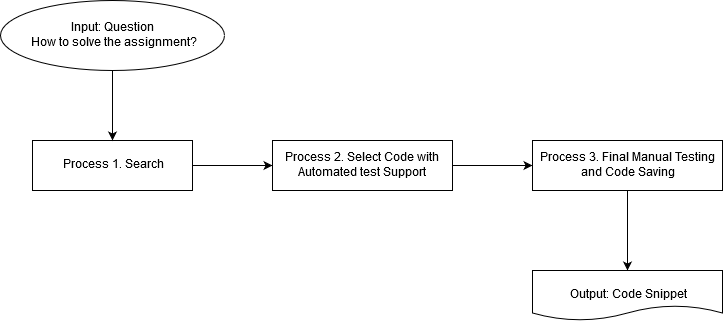
\includegraphics[width=0.5\textwidth]{./figures/Process_Flow.png}
Our targeted users do not know how to code.

Assignment Helper gives the code.
\caption{Process Flow of Assignment Helper}
\label{fig_process_flow}
\end{figure}


\textbf{Getting Started}

\subsection{Setting - Easy Installation}

\begin{enumerate}
  \item Description
  \begin{itemize}
    \item Executable without installation to facilitate ease of use
    \item Works like portable utility
    \item Basic files only provide barebone program
    \begin{itemize}
      \item Programming language to search need be installed later
    \end{itemize}
  \end{itemize}
  \item Process(or I/O)
  \begin{enumerate}
    \item Download files from website
  \end{enumerate}
\end{enumerate}
\textit{}


\subsection{Setting - Configuration Window}

\begin{enumerate}
  \item Description
  \begin{itemize}
    \item Basic program is not able to use without installing programming language
    \item Provide check window
    \begin{itemize} 
      \item Check each window to install a language pack for a certain language 
    \end{itemize}
  \end{itemize}
  \item Process(or I/O)
  \begin{enumerate}
    \item Input: Opening conf.exe
    \item Output: Show conf.exe
  \end{enumerate}
\end{enumerate}

\textit{}

\subsection{Setting - Installing Language Pack}
\begin{enumerate}
  \item Description
  \begin{itemize}
    \item Basic program is not able to use without installing programming language
    \item Provide check window
    \begin{itemize}
      \item Check each window to install a language pack for a certain language 
    \end{itemize}
  \end{itemize}
  \item Process(or I/O)
  \begin{enumerate}
    \item Input: Selecting language packs and proceed 
    \item Output: Pack install on the hard disk
  \end{enumerate}
\end{enumerate}


\textit{}
\subsection{Instruction - README}
\begin{enumerate}
  \item Description
  \begin{itemize}
    \item Provide README file to give basic instruction
  \end{itemize}
  \item Process(or I/O)
  \begin{enumerate}
    \item N/A
  \end{enumerate}
\end{enumerate}


\textit{}

\subsection{Instruction - Basic Tutorial}
\begin{enumerate}
  \item Description
  \begin{itemize}
    \item Give demo-like tutorial on the very first run
  \end{itemize}
  \item Process(or I/O)
  \begin{enumerate}
    \item Input: Clicking tutorial on main window
    \item Input2: Initial program execution
    \item Output: Install selected pack on the hard disk
  \end{enumerate}
\end{enumerate}


\textit{}

\subsection{Instruction - On the Fly}
\begin{enumerate}
  \item Description
  \begin{itemize}
    \item Give tooltips on buttons
  \end{itemize}
  \item Process(or I/O)
  \begin{enumerate}
    \item Input: Hovering on a button for 3 seconds
    \item Output: Show up a tool tip
  \end{enumerate}
\end{enumerate}

\textit{}

\textbf{Execution}

\subsection{Execution}
\begin{enumerate}
  \item Description
  \begin{itemize}
    \item Executing the main program
  \end{itemize}
  \item Process(or I/O)
  \begin{enumerate}
    \item Opening the main program(helper.exe)
    \item Program(Process1. UI) shows up within 1 minute
  \end{enumerate}
\end{enumerate}

\textit{}

\subsection{Closing Whole Program}
\begin{enumerate}
  \item Description
  \begin{itemize}
    \item Closing Whole Program
  \end{itemize}
  \item Process(or I/O)
  \begin{enumerate}
    \item Clicking X window on search UI
    \item Program closing
  \end{enumerate}
\end{enumerate}
\textit{}


%프롬프트
\textbf{Process 1. Searching}


\textit{}
\begin{figure}[h]
\centering
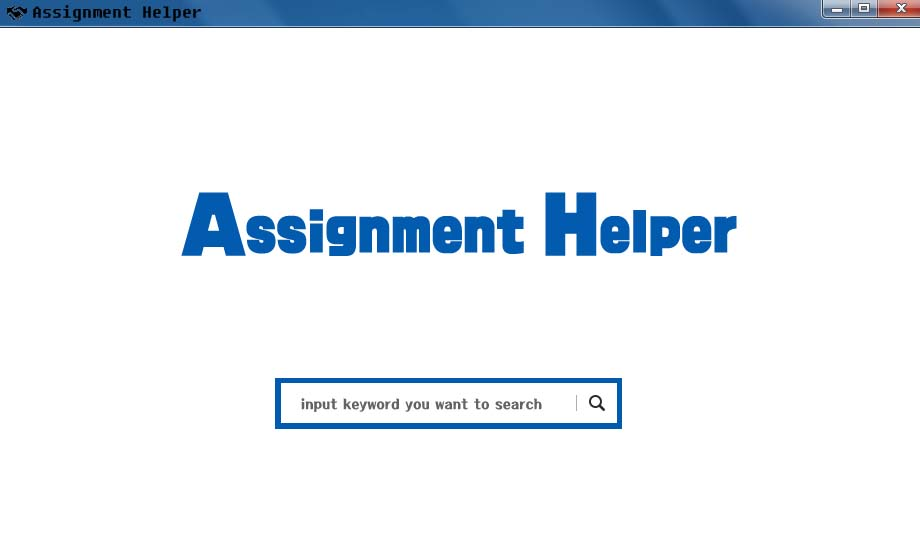
\includegraphics[width=0.5\textwidth]{./figures/UI_main.jpg}
%text slot
\caption{Concept Image of Search Window}
\label{fig_concept_main}
\end{figure}


\subsection{Search - UI}
\begin{enumerate}
\item Description
\begin{itemize}
   \item Give instinctive search home
\end{itemize}
\item Process(or I/O)
  \begin{enumerate}
     \item Clicking search button on search UI
     \item Search begins
  \end{enumerate}
\end{enumerate}
\textit{}

\subsection{Search – History}
\begin{enumerate}
\item Description
\begin{itemize}
   \item Show searh history
\end{itemize}
\item Process(or I/O)
  \begin{enumerate}
     \item Output: Show up top 5 from search history list
  \end{enumerate}
\end{enumerate}
\textit{}

\subsection{Search – Option}
\begin{enumerate}
\item Description
\begin{itemize}
  \item Choose in what programming language result represent
  \begin{itemize}
     \item Show language option buttons
  \end{itemize}
\end{itemize}
\item Process(or I/O)
  \begin{enumerate}
    \item Input: click on a python button 
    \item Output: Show result on a python language 
    \item Input: click on a C button 
    \item Output: Show result on a C language 
    \item Input: click on a C++ button 
    \item Output: Show result on a C++ language 
  \end{enumerate}
\end{enumerate}
\textit{}

\subsection{Search – Auto Completion}
\begin{enumerate}
\item Description
\begin{itemize}
  \item Show match from search ketwords.csv
\end{itemize}
\item Process(or I/O)
  \begin{enumerate}
     \item Input: Each letters typed
    \item Output: Show all match words from search ketwords.csv
  \end{enumerate}
\end{enumerate}
\textit{}

\subsection{Request Submission by Key Press}
\begin{enumerate}
\item Description
\begin{itemize}
  \item Submit request by typing enter 
\end{itemize}
\item Process(or I/O)
  \begin{enumerate}
  \item Input: type enter key
  \item Output: Submit request
  \end{enumerate}
\end{enumerate}
\textit{}

\subsection{Request Submission by Clicking}
\begin{enumerate}
\item Description
\begin{itemize}
  \item Submit request by click 
\end{itemize}
\item Process(or I/O)
  \begin{enumerate}
     \item Input: mouse click
    \item Output: Submit request
  \end{enumerate}
\end{enumerate}
\textit{}

\subsection{Request Submission - Waiting UI}
\begin{enumerate}
\item Description
\begin{itemize}
  \item Halt user interface while submission 
\end{itemize}
\item Process(or I/O)
  \begin{enumerate}
     \item input: Submit request 
     \item Output: Freeze UI
  \end{enumerate}
\end{enumerate}
\textit{}

\subsection{Request Submission - Abort}
\begin{enumerate}
\item Description
   \begin{itemize}
  \item User press cancel
  \item Error occurs
  \item End submission
  \item Back to search window 
\end{itemize}
\item Process(or I/O)
  \begin{enumerate}
     \item input: Click cancel button
     \item input: Error occurs 
     \item Output: Stop submission
     \item Output: Back to start page
  \end{enumerate}
\end{enumerate}
\textit{}

\subsection{Request Submission – Extracting Keyword}
\begin{enumerate}
\item Description
\begin{itemize}
  \item Extract keywords from submitted  
\end{itemize}
\item Process(or I/O)
  \begin{enumerate}
     \item input: Submit request 
     \item Output: Freeze UI
  \end{enumerate}
\end{enumerate}
\textit{}

\subsection{Request Processing - Crawling(Stackoverflow)}
\begin{enumerate}
\item Description
\begin{itemize}
  \item Crawl popular codes
  \item Organize codes by keywords
  \item Process(or I/O) 
  \item Crawl Stackoverflow by keywords.csv
  \item Give code with popularity over 3/5 to code page
\end{itemize}
\begin{enumerate}
     \item Make keyword a key 
     \item Organize code page by keyword order
  \end{enumerate}
\end{enumerate}
\textit{}

\subsection{Request Processing - Crawling(Google)}
\begin{enumerate}
\item Description

\begin{itemize} 
  \item Crawl popular codes
  \item Organize codes by keywords
  \item Process(or I/O)
  \item Crawl Google by keywords.csv
  \item Give code with popularity over 3/5 to code page
\end{itemize}
  \begin{enumerate}
     \item Make keyword a key 
     \item Organize code page by keyword order
  \end{enumerate}
\end{enumerate}
\textit{}

\subsection{Request Processing - Detect Code Part}
\begin{enumerate}
\item Description
  \begin{itemize}
    \item Do encoding test to know if it is right code
  \end{itemize}
  \item Process(or I/O)
  \begin{enumerate}
    \item Encode code page
    \item output: error code
  \end{enumerate}
\end{enumerate}
\textit{}


\subsection{Request Completed - UI}
\begin{enumerate}
  \item Description
  \begin{itemize}
    \item Give code page to selection
  \end{itemize}
  \item Process(or I/O)
  \begin{enumerate}
    \item Give all crawled code page to selection phase
  \end{enumerate}
\end{enumerate}

\textit{}

\textbf{Process 2. Code Selction}


\textit{}
\begin{figure}[h]
\centering
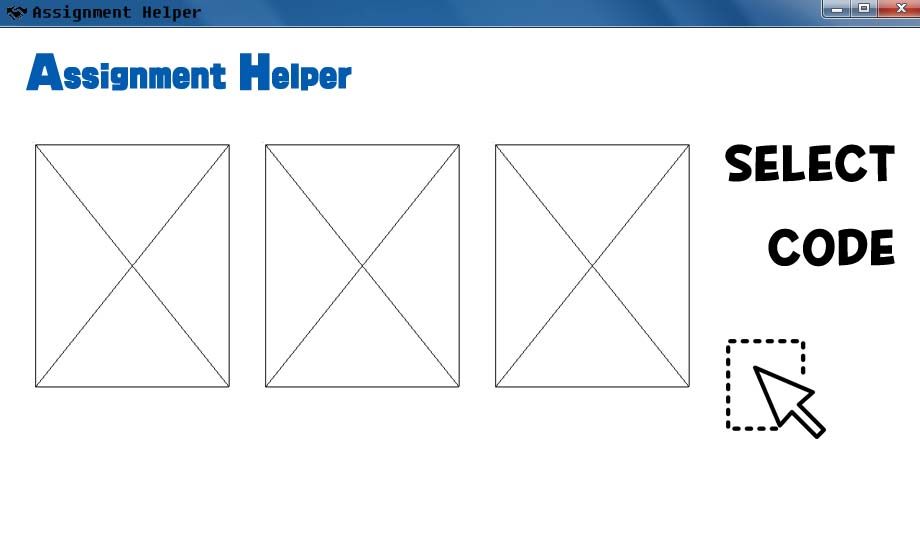
\includegraphics[width=0.5\textwidth]{./figures/UI_code_select.jpg}
%text slot
\caption{Concept Image of Code Select Window}
\label{fig_concept_code_select}
\end{figure}


\subsection{Code Selection - Basic UI}

\begin{enumerate}
  \item Description
  \begin{itemize}
    \item User should select code among results before program starts other process
  \end{itemize}
  \item Process(or I/O)
  \begin{enumerate}
    \item Clicking code among results
    \item Next process starts within 5 seconds
  \end{enumerate}
\end{enumerate}


\textit{}

\subsection{Auto Compile Test - Requesting}

\begin{enumerate}
  \item Description
  \begin{itemize}
    \item Right after user selects code, program is compiling the code(See Figure~\ref{fig_concept_code_compile} )
  \end{itemize}
  \item Process(or I/O)
  \begin{enumerate}
    \item Input : Text that user chose
    \item Output: Test. Program format
  \end{enumerate}
\end{enumerate}

\textit{}
\begin{figure}[h]
\centering
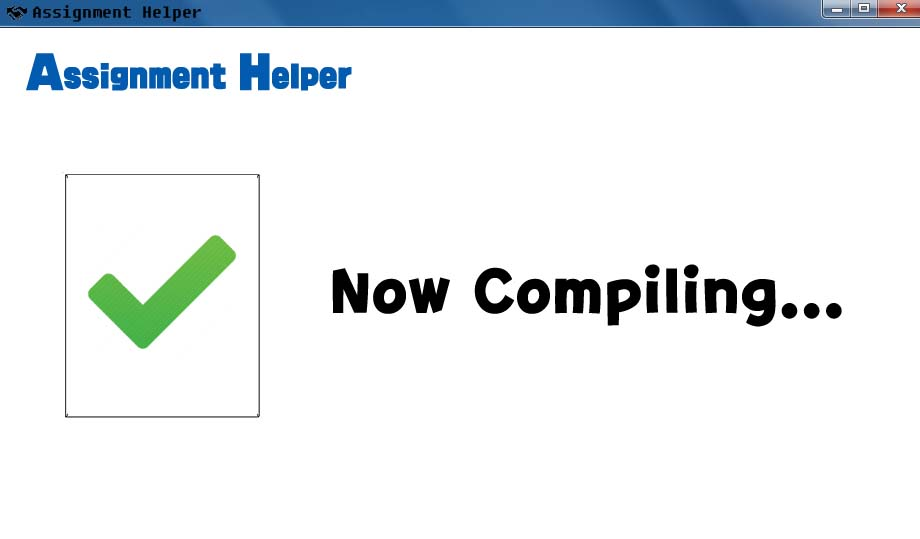
\includegraphics[width=0.5\textwidth]{./figures/UI_code_validation.jpg}
%text slot
\caption{Concept Image of Code Compiling}
\label{fig_concept_code_compile}
\end{figure}

\textit{}

\subsection{Auto Compile Test - Success}

\begin{enumerate}
  \item Description
  \begin{itemize}
    \item If compiling is finished successfully, without error code, code box goes green
  \end{itemize}
  \item Process(or I/O)
  \begin{enumerate}
    \item Waiting for finish of compiling
    \item Check whether error code exists or not (No error code = Success)
  \end{enumerate}
\end{enumerate}

\textit{}

\subsection{Auto Compile Test - Failure}

\textit{}
\begin{figure}[h]
\centering
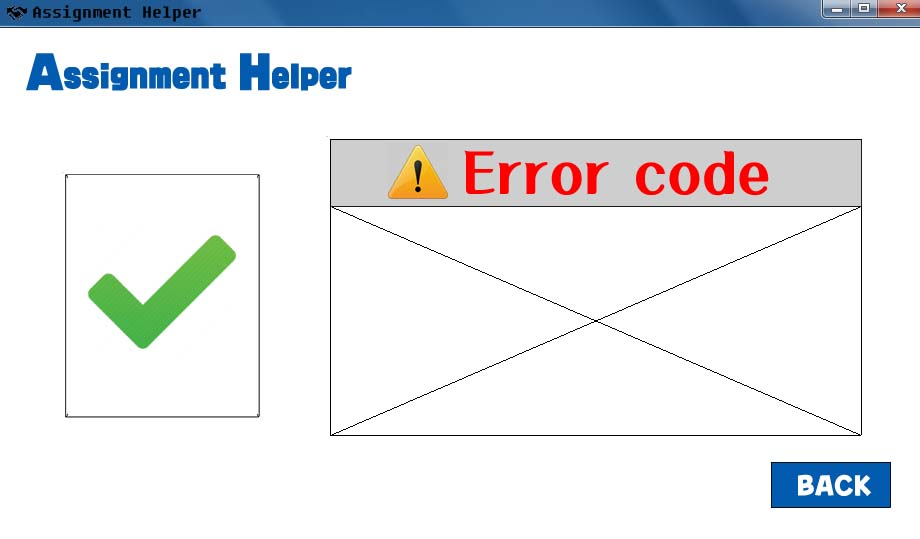
\includegraphics[width=0.5\textwidth]{./figures/UI_code_validation_fail.jpg}
%text slot
\caption{Concept Image of Code Testing Failure}
\label{fig_concept_fail}
\end{figure}


\begin{enumerate}
  \item Description
  \begin{itemize}
    \item If there is error code after compiling, program shows the error code to user (see Figure~\ref{fig_concept_fail})
  \end{itemize}
  \item Process(or I/O)
  \begin{enumerate}
    \item Waiting for finish of compiling
    \item Show error code result to user
    \item Enable users to edit codes if they can find the error.
  \end{enumerate}
\end{enumerate}

\textit{}

\subsection{Auto Compile Test - Edit Code Snippet}
\begin{enumerate}
  \item Description
  \begin{itemize}
    \item When the auto compile test ended with error, users are able to edit code manually
  \end{itemize}
  \item Process(or I/O)
  \begin{enumerate}
    \item Input: Error signal from auto compile test
    \item Output: Enabling users to edit code
  \end{enumerate}
\end{enumerate}


\textit{}


\subsection{Cancellation(2) - Clicking Return Button}
\begin{enumerate}
  \item Description
  \begin{itemize}
    \item After finishing compiling or during compiling, user can go back with clicking return button
  \end{itemize}
  \item Process(or I/O)
  \begin{enumerate}
    \item Clicking return button
    \item Go back to the code selection window
  \end{enumerate}
\end{enumerate}
\textit{}


\subsection{Cancellation(2) - Cliking X Window Button}
\begin{enumerate}
  \item Description
  \begin{itemize}
    \item After finishing compiling or during compiling, user can exit program
  \end{itemize}
  \item Process(or I/O)
  \begin{enumerate}
    \item Clicking X window button
    \item Terminate program
  \end{enumerate}
\end{enumerate}
\textit{}


\subsection{Selection - Proceed without testing}
%put warning window
\begin{enumerate}
  \item Description
  \begin{itemize}
    \item Users are able to procced without auto compile test
    \item Autocompile tested bits off
  \end{itemize}
  \item Process(or I/O)
  \begin{enumerate}
    \item Users click next button
    \item Proceed to process 3
  \end{enumerate}
\end{enumerate}
\textit{}


\subsection{Prompt - Cancellation}
\begin{enumerate}
  \item Description
  \begin{itemize}
    \item When user requests cancellation, prompt window appears, reconfirming cancellation
  \end{itemize}
  \item Process(or I/O)
  \begin{enumerate}
    \item Clicking Return or X window button
    \item Reconfirming cancellation, Yes or No
  \end{enumerate}
\end{enumerate}
\textit{}



\subsection{Prompt - Proceed}
\begin{enumerate}
  \item Description
  \begin{itemize}
    \item Before proceeding compiling, prompt window appears, reconfirming proceeding it
  \end{itemize}
  \item Process(or I/O)
  \begin{enumerate}
    \item Clicking code
    \item Reconfirming proceeding, Yes, or No
  \end{enumerate}
\end{enumerate}
\textit{}


\textbf{Process 3. Manual Testing and Result Saving}


\textit{}
\begin{figure}[h]
\centering
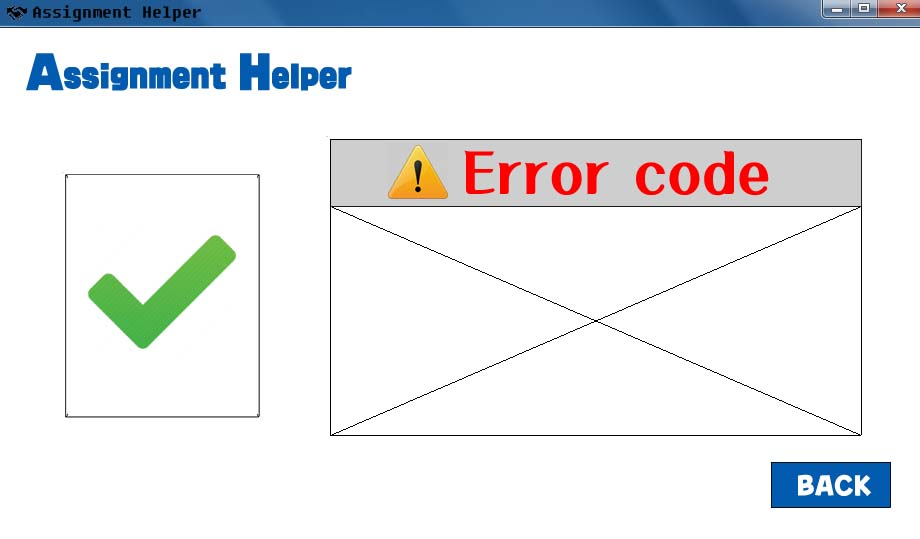
\includegraphics[width=0.5\textwidth]{./figures/UI_code_validation_fail.jpg}  
%text slot
\caption{Concept Image of Code Validation}
\label{fig_concept_validation_manual}
\end{figure}


\subsection{Result - UI}
\begin{enumerate}
  \item Description
  \begin{itemize}
    \item Showing result and providing process check and copy function to user (see Figure~\ref{fig_concept_validation_manual}.
  \end{itemize}
  \item Process(or I/O)
  \begin{enumerate}
    \item 3 button – Input, Output, Copy Code
  \end{enumerate}
\end{enumerate}
\textit{}

\subsection{Process Checking - Input \& Output}
\begin{enumerate}
  \item Description
  \begin{itemize}
    \item User can check whether code is what they wanted or not through manual checking process
    \item Once user pushes input value into the program, they can see there is expected output or not.
  \end{itemize}
  \item Process(or I/O)
  \begin{enumerate}
    \item Input: Input value into program formed with selected code
    \item Output: Print output from pushed input
  \end{enumerate}
\end{enumerate}
\textit{}


\subsection{Copy Code}

\begin{enumerate}
  \item Description
  \begin{itemize}
    \item Providing copy the whole code which is selected, easily
  \end{itemize}
  \item Process(or I/O)
  \begin{enumerate}
    \item Clicking copy button
    \item Copy selected code on the clipboard
  \end{enumerate}
\end{enumerate}
\textit{}



\subsection{Cancellation(4) - Clicking Return Button}
\begin{enumerate}
  \item Description
  \begin{itemize}
    \item User can go back with clicking return button
  \end{itemize}
  \item Process(or I/O)
  \begin{enumerate}
    \item Clicking return button
    \item Go back to the code selection window
  \end{enumerate}
\end{enumerate}
\textit{}


\subsection{Cancellation(4) - Cliking X Window Button}
\begin{enumerate}
  \item Description
  \begin{itemize}
    \item User can exit program
  \end{itemize}
  \item Process(or I/O)
  \begin{enumerate}
    \item Clicking X window button
    \item Program closing
  \end{enumerate}
\end{enumerate}
\textit{}

\section{Architecture Design and Implementation} % (fold)
\label{sec:architecture_design_and_implementation}

\subsection{Overall architecture} % (fold)
\label{sub:overall_architecture}

see Figure~\ref{overall}

% subsection overall_architecture (end)

\subsection{Directory Organization} % (fold)
\label{sub:directory_organization}

\begin{table}[h]
\renewcommand{\arraystretch}{1.3}
\caption{Directory Organization}
\label{table:directory_org}
\centering
\begin{adjustbox}{width=0.5\textwidth}
\small
\begin{tabular}{c||c||c}
\hline
\bfseries Directory & \bfseries File Names & \bfseries Module Names \\
\hline\hline
project/src/keyword/  & \parbox[t]{5cm}{synonym\_test.csv \\ keyword\_search.py \\ topic\_analysis.py} & \parbox[t]{5cm}{keyword\_search}\\
\hline
project/src/crawling/ & \parbox[t]{5cm}{crawling\_common.py \\ crawling\_stack.py \\ crawling\_google.py} & \parbox[t]{5cm}{get\_code}\\
\hline
project/src/comp\_exec/ &\parbox[t]{5cm}{error\_argument\_C++.py \\ execution\_C++.py \\ error\_argument\_py.py \\ execution\_py.py \\ ... } & \parbox[t]{5cm}{validation}\\
\hline
project/src/GUI/ & \parbox[t]{5cm}{search.py \\candidates.py \\ compiling.py \\ error.py \\ success.py} & \parbox[t]{5cm}{GUI}\\
\hline

\end{tabular}
\end{adjustbox}
\end{table}

% subsection directory_organization (end)
\textbf{Module Description}

\subsection{keyword - keyword\_search} % (fold)
\label{sub:keyword_search}
\begin{figure}[ht]
\centering
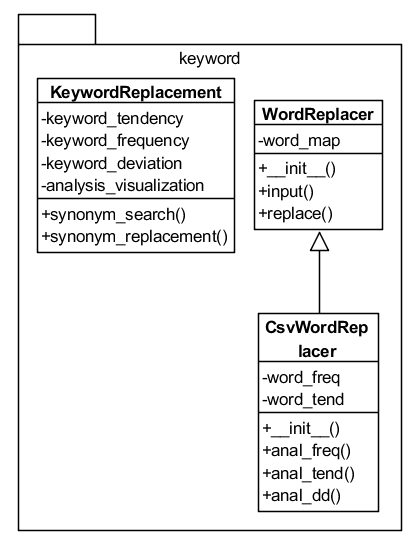
\includegraphics[width=0.5\textwidth]{./figures/keyword_search.png}
%description of module get\_info
\caption{Description of module \textit{keyword\_search}}
\label{keyword_search}
\end{figure}


This module is to take real language from user in sentence or words, split up, and replace them to keywords for search. Our program is to detect keywords from natural language, and make coded files for output. For that, a csv file for keywords is needed. If this list of keywords is too short, all it can make is an error sign. So, we first made 2000 words for key, and make it extend. What we need for search a word in some sentences is first, split function. By that, we can save our resources for replacement, reduce error cases, or decrease misunderstanding. Then it replaces natural language to limited number of keyword. Those keywords are sent to next stage. And it analyzes frequency, deviation, and tendency of keyword composition for later use. The synonym\_word.csv is for those keywords, but there will be needs of complement. So, with analysis of keywords, the csv file extends. 


see Figure~\ref{keyword_search}
% subsection keyword_search (end)

\subsection{get\_code - Crawling and Selecting} % (fold)
\label{sub:get_code}
\begin{figure}[ht]
\centering
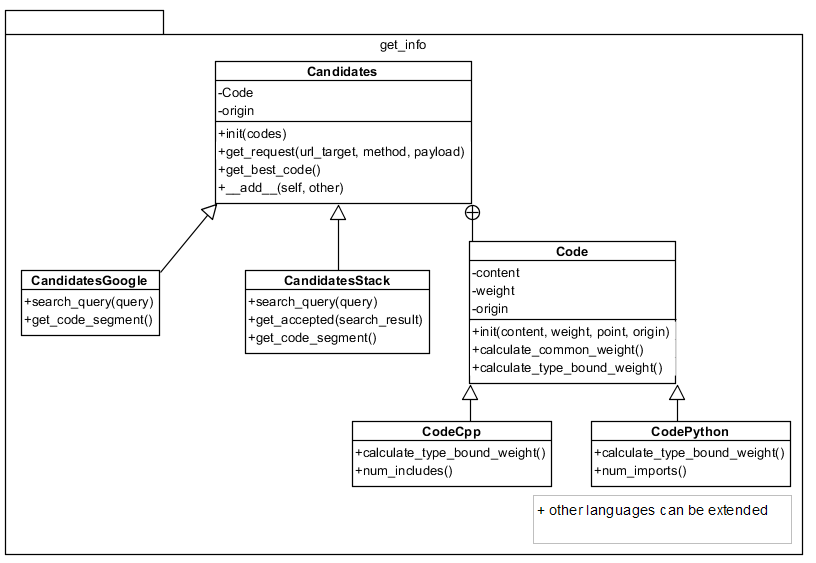
\includegraphics[width=0.5\textwidth]{./figures/get_info.png}
%description of module get\_info
\caption{Description of module \textit{get\_info}}
\label{get_info}
\end{figure}

This module search for appropriate codes using keywords from the \textit{query} module.
\textit{get\_code} imports \textit{requests} for query requesting to the server, mostly using REST API supported from forums.
For raw html files, the module imports \textit{beautifulsoup4} package to parse the code.
After crawling codes from sites, this module also evaluates the quality of the code.


see Figure~\ref{get_info}
% subsection search_crawling (end)

\subsection{validation - Compling and Execution} % (fold)
\label{sub:validation}

\label{sub:validation}
\begin{figure}[ht]
\centering
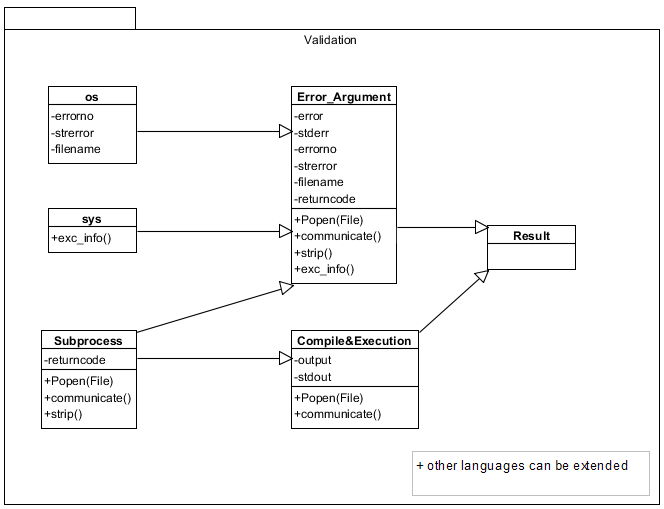
\includegraphics[width=0.5\textwidth]{./figures/comp_exec.png}
%description of module get\_info
\caption{Description of module \textit{validation}}
\label{validation}
\end{figure}
This module is to take cpp file generated after parsing codes, then compile, and execute it.
It imports \textit{subprocess}, which makes python freely handle other programming language.
It creates command with Popen function in subprocess, and then executes it with communicate function in subprocess.
It compiles test.cpp using g++ and executes it using "./test" command
Error handling is made by error exception method. 
At this point, it imports os, sys, and subprocess. 
Each of these catches error which they can handle.
The os uses errorno, strerror, and filename.
The sys uses exc\_info() function, and the subprocess uses returncode and strip() function.
Then Error\_Argument prints out error caused within os, sys, and process.

see Figure~\ref{validation}
% subsection validation (end)

\subsection{GUI} % (fold)
\label{sub:gui}
\begin{figure}[ht]
\centering
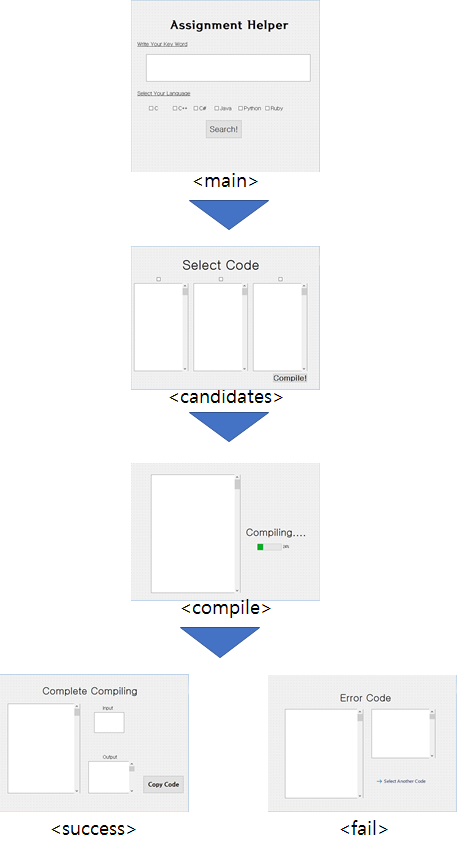
\includegraphics[width=0.5\textwidth]{./figures/gui_overall.png}
%description of module get\_info
\caption{Description of module \textit{gui}}
\label{gui}
\end{figure}
GUI consists of 5 windows corresponds to each procedure.
Firstly, the \textit{main} window provides search.
After clicking the search, the program executes \textit{keyword\_search} and then window moves to \textit{search\_result} window.
\textit{search\_result} window has candidates from \textit{get\_info} module.

Clicking \textit{compile} button on the  \textit{search\_result} window will execute compile.
Compile is done by \textit{validation} module. After compiling, the program shows either \textit{success} or \textit{fail} window


see Figure~\ref{gui}
% subsection gui (end)


% section architecture_design_and_implementation (end)


\section{Use Case} % (fold)
\label{sec:use_case}

\subsection{install}
This use case specifies the way user install the program

\begin{itemize}
  \item download the file from the link
  \item auto extractor will unzip the program
  \item show pragram installed finished display
\end{itemize}
\textit{}



\subsection{first run the program}
This use case presents how the program will act when the program is run very first time
\begin{itemize}
  \item initial running the program
  \item show up the configuration window(conf.exe)
  \item after configuration done, do the tutorial
\end{itemize}
\textit{}



\subsection{do the tutorial}
This use case specifies how the program will act when user do the tutorial
\begin{itemize}
  \item clicking the tutorial button on main window or initial setting 
  \item play the tutorial movie(tut.mov)
  \item after playing the tutorial, close the tut.mov
\end{itemize}
\textit{}



\subsection{open configuration window}
This use case specifies how the configuration window looks like when the user opens the configuration window
\begin{itemize}
  \item initial running the program or double clicking on conf.exe
  \item open a checkbox gui
  \item the checkbox gui has languages to be installed
\end{itemize}
\textit{}



\subsection{check the languages and confirm installation}
This use case specifies how the program should act in the configuration window. In the configuration window, the user can easily install language packs from server.
\begin{itemize}
  \item check language packs to install / uncheck languages to uninstall
  \item click install button to install and uninstall selected ones
\end{itemize}
\textit{}



\subsection{open readme}
This use case describes about opening the readme file.
\begin{itemize}
  \item open a readme file which gives basic installation
\end{itemize}
\textit{}



\subsection{run the program(main.exe)}
This use case specifies of initializing the program when the user executes the program.
\begin{itemize}
  \item running the program
  \item open the main window(search window)
\end{itemize}
\textit{}



\subsection{tooltips}
This use case specifies about how the user enables the tooltips
\begin{itemize}
  \item hanging mouse on the buttons for 3 seconds
  \item show the tooltips
  \item tooltip disappear 1 seconds after mouse hovering finished
\end{itemize}
\textit{}



\subsection{view search history}
This use case specifies about viewing search history. User can view the search history and replicates the search result using search history.
\begin{itemize}
  \item clicking search history button
  \item show search history pane
\end{itemize}
\textit{}


\subsection{enter a query}
This use case sepecfies how users can search their questions. The users first select the language and then search on window
\begin{itemize}
  \item enter a query on the search window
  \item while entering a query, keep run auto completion
  \item show the auto completion result
  \item select language to search
  \item uninstalled languages are greyed out
\end{itemize}
\textit{}



\subsection{submit the query}
This use case specifies the procedures when submitting the query
\begin{itemize}
  \item click 'search' button
  \item run, query extracting module
  \item run, \textit{get\_code} module based on the result
  \item show the candidates window
\end{itemize}
\textit{}


\subsection{select code}
This use case specifies about how user can interact with \textit{candidates} window. This is the main interaction with the program.
\begin{itemize}
  \item view each code to compile
  \item the user evaluates codes
  \item click code that the user things the best suitable.
\end{itemize}
\textit{}



\subsection{modify code}
This use case specifies about modifiying the code if the user wants to.
\begin{itemize}
  \item the user decide whether the codes needs to be refined
  \item click on the code
  \item editing the code
  \item press enter to confirm
\end{itemize}
\textit{}



\subsection{compile code}
This use case specifies about compiling the code, when user clicks copile button.
\begin{itemize}
  \item after select and modify, user press compile button
  \item validation module executes the compile process
  \item show the result of compiling either \textit{success} or \textit{fail}
\end{itemize}
\textit{}



\subsection{pop up fail window}
This use case specifies when the compile fails, shows error result.
\begin{itemize}
  \item failure of the compiling triggers the fail window
  \item show the fail window
  \item fail window shows errors
\end{itemize}
\textit{}



\subsection{pop up success window}
This use case specifies when the compile succeed, shows copy code window.
\begin{itemize}
  \item pops up the window
  \item the success window provides to test input and output
  \item the success window also provides copying code
\end{itemize}
\textit{}



\subsection{test input}
This use case specifies about testing more input using \textit{validation} module.
\begin{itemize}
  \item put input on the input textbox
  \item click on the test button
  \item outcome will show the result with the program
\end{itemize}
\textit{}



\subsection{copy code}
This use case specifies when the user wants to save result, this provides the way to save the result.
\begin{itemize}
  \item press copy code button
  \item code will be copied to the clipboard
\end{itemize}
\textit{}



\subsection{click x button}
This use case specifies how the program act when x buttons are clicked
\begin{itemize}
  \item click x button
  \item pops prompt window that asks about the cancellation
  \item cancel all procedure and go back to the first search window
\end{itemize}
\textit{}



\subsection{program exit}
This use case specifies how to close the program.
\begin{itemize}
  \item click x button on main(search) window
  \item program terminates
\end{itemize}
\textit{}



% section use_case (end)

\begin{figure*}
\centering
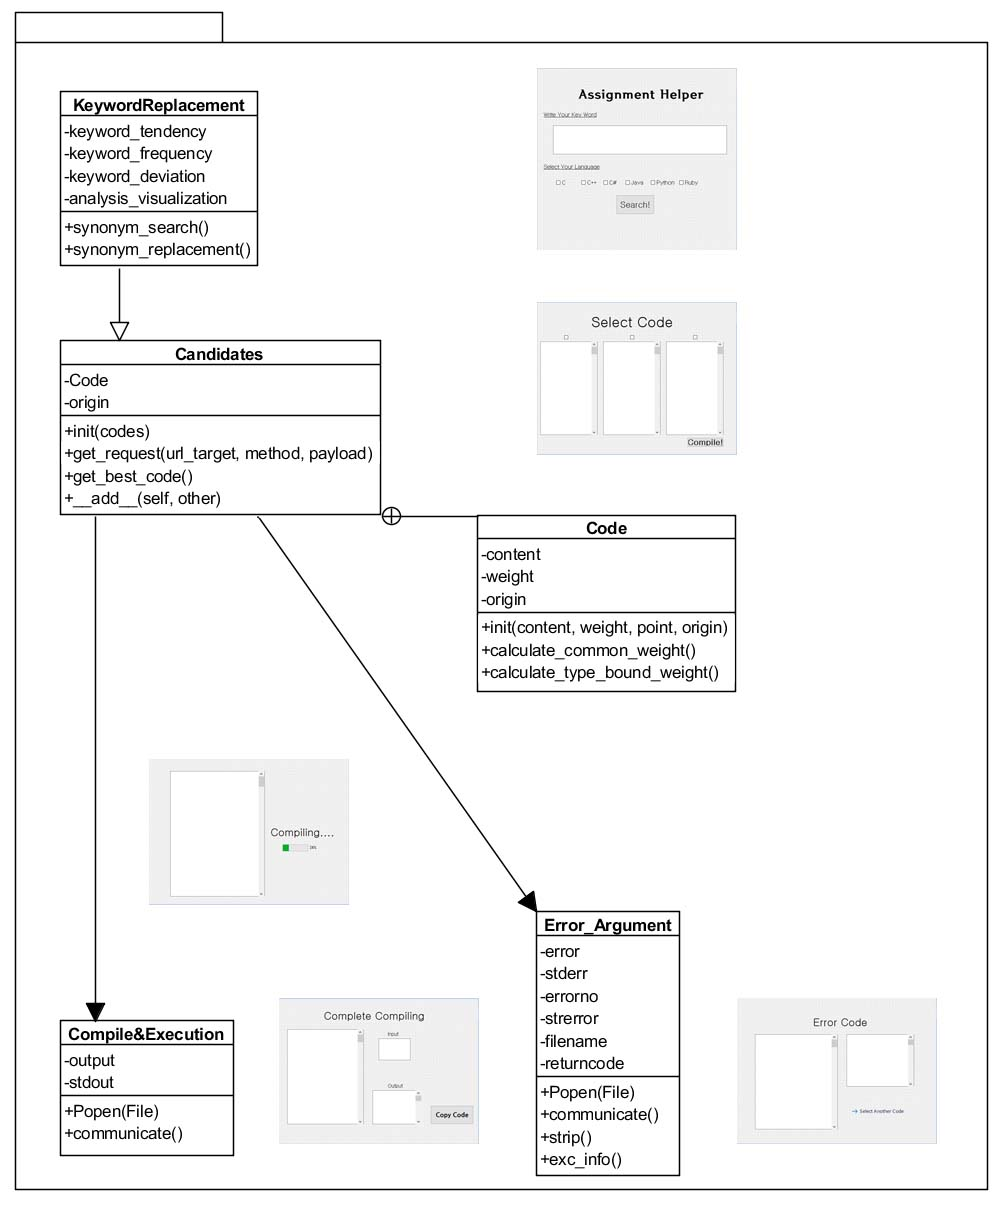
\includegraphics[width=1\textwidth]{./figures/overall_arch.jpg}
%description of module get\_info
\caption{Description of Overall Architecture}
\label{overall}
\end{figure*}


% ''-------------end of the document-------------------''
% % figure example --------------
% \begin{figure}[h]
% \centering
% 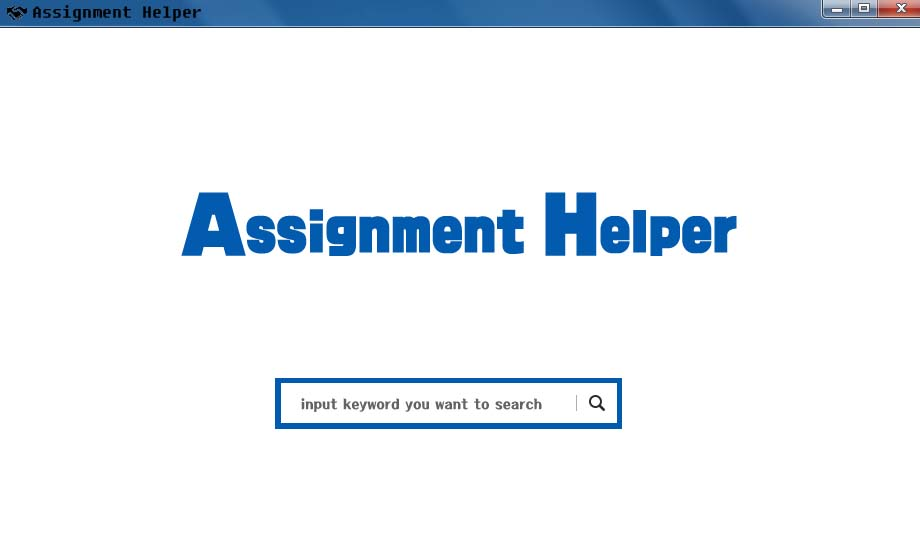
\includegraphics[width=0.5\textwidth]{./figures/UI_main.jpg}
% %text slot
% \caption{Example Example.}
% \label{fig_sim}
% \end{figure}

% section specifications (end)
% \begin{thebibliography}{1}

% \bibitem{IEEEhowto:kopka}
% H.~Kopka and P.~W. Daly, \emph{A Guide to \LaTeX}, 3rd~ed.\hskip 1em plus
%   0.5em minus 0.4em\relax Harlow, England: Addison-Wesley, 1999.

% \end{thebibliography}




% that's all folks
\end{document}


